% This is samplepaper.tex, a sample chapter demonstrating the
% LLNCS macro package for Springer Computer Science proceedings;
% Version 2.20 of 2017/10/04
%
\documentclass[runningheads]{llncs}
%
\usepackage{graphicx}
\usepackage{float}
\usepackage{wrapfig}

% Used for displaying a sample figure. If possible, figure files should
% be included in EPS format.
%
% If you use the hyperref package, please uncomment the following line
% to display URLs in blue roman font according to Springer's eBook style:
% \renewcommand\UrlFont{\color{blue}\rmfamily}
\usepackage{color, colortbl}
\definecolor{navy}{RGB}{0,0,205}
\definecolor{darkred}{RGB}{178,34,34}
\definecolor{darkblue}{RGB}{0,10,230}
\definecolor{green}{RGB}{20,180,20}
\definecolor{verylightgray}{RGB}{220,220,220}

% colors fo rules
\definecolor{darkgreen}{RGB}{0,153,0}
\definecolor{darkorange}{RGB}{204,102,0}
\newcommand{\W}{\textbf{W}$^2$ }
\newcommand{\dollar}{\mbox{\textdollar}}
\definecolor{campusgold}{RGB}{194,142,14}
\definecolor{headlinegold}{RGB}{152, 112, 13}
\definecolor{coalgray}{RGB}{77,64,56}
\definecolor{moongray}{RGB}{186,168,146}
\definecolor{everblue}{RGB}{91,104,112}
\definecolor{slayterblue}{RGB}{124,166,192}
\definecolor{ameliablue}{RGB}{163,214,215}
\definecolor{landgreen}{RGB}{8,92,17}
\definecolor{rossgreen}{RGB}{132,158,42}
\definecolor{celerygreen}{RGB}{195,190,11}
\definecolor{springgreen}{RGB}{233,228,91}
\definecolor{oakenbrown}{RGB}{107,69,52}
\definecolor{bellbrick}{RGB}{199,108,20}
\definecolor{mackeyorange}{RGB}{255,155,26}
\definecolor{yellowwalk}{RGB}{255,209,0}
\definecolor{fountainteal}{RGB}{46,175,155}
\definecolor{pappyspurple}{RGB}{173,31,101}

\usepackage[round]{natbib}
\usepackage{amsmath}
\usepackage{stmaryrd}
\usepackage{amsfonts}
\usepackage{listings}
\lstdefinelanguage{Scala}%
{morekeywords={abstract,%
  case,catch,char,class,%
  def,else,extends,final,finally,for,%
  if,import,implicit,%
  match,module,%
  new,null,%
  object,override,%
  package,private,protected,public,%
  for,public,return,super,%
  this,%throw,throws,
  trait,try,type,throw,%
  val,var,%
  with,while,%
  yield,%
  },%
  sensitive,%
  morecomment=[l]//,%
  morecomment=[s]{/*}{*/},%
  morestring=[b]",%
  morestring=[b]',%
  showstringspaces=false%
  inputencoding=utf8,
  extendedchars=true,
  moredelim=[is][\overbar]{`}{`},
  moredelim=[is][\sout]{~}{~},
  escapechar=@
}[keywords,comments,strings]%

\definecolor{dkgreen}{rgb}{0,0.6,0}
\definecolor{gray}{rgb}{0.5,0.5,0.5}
\definecolor{mauve}{rgb}{0.58,0,0.82}
\definecolor{violet}{rgb}{0.53, 0.0, 0.69}
\definecolor{violet2}{rgb}{0.93, 0.51, 0.93}
\definecolor{backcolour}{rgb}{0.95,0.95,0.92}

\lstset{
  language=Scala,
  basicstyle=\ttfamily,
  keywordstyle={\bfseries\color{violet}},
  commentstyle=\color{dkgreen},
  stringstyle=\color{blue},
  mathescape
}
\usepackage[T1]{fontenc}
\usepackage[scaled=0.9]{beramono}

\makeatletter
\newcommand{\printfnsymbol}[1]{%
  \textsuperscript{\@fnsymbol{#1}}%
}
\makeatother

\begin{document}
%
\title{\W: From Static Graph to Responsive HTML}
%
%\titlerunning{Abbreviated paper title}
% If the paper title is too long for the running head, you can set
% an abbreviated paper title here
%
\author{Shangyin Tan\thanks{equal contribution} \and
Tiger Tang\printfnsymbol{1}}
%
% First names are abbreviated in the running head.
% If there are more than two authors, 'et al.' is used.
%
\institute{Purdue University\\
\email{\{tan279,tang426\}@purdue.edu}}
%
\maketitle % typeset the header of the contribution
%
\begin{abstract}
  We present a novel approach to synthesize and generate a nested and responsive UI layout from a wireframe, a common tool used by UI/UX designers to draft their design of a client application. Given the wireframe design of an application's layout in absolute coordinates, \W synthesizes an HTML file that when rendered by any modern browser, not only places the components in their original positions, but also automatically adapts to changes in the viewer's screen size using modern HTML and CSS techniques. Furthermore, the resulting HTML has a clearly defined parent-child hierarchy, enabling the application developer to iterate and detail it quickly. Preliminary benchmark results show that W2 is able to synthesize an absolute wireframe layout consisting of 200+ rectangles into an HTML hierarchy tree of depth 5 in under 2ms.
\keywords{Program Synthesis  \and Web Development \and User Interface}
\end{abstract}
%
%
%
\section{Introduction}
UI/UX design plays an important role in most software applications. It allows software users to interact with the software functions and perform the designated tasks in an intuitive and effective way. The usual client application development cycle is as below: the UI/UX designer first designs the application layout, then provides it in image format to the application developer, who then writes code that when rendered resembles the design. However, the latter task is often time-consuming and error-prone. For instance, the spacings between the layout elements, referred to as margins, are often not accurately implemented by the application programmer, either because they are not explicitly stated in the design or such process simply takes too much time, so that the programmer uses estimated values instead.

Furthermore, as the popularity of mobile devices grows, a single fixed layout is no longer sufficient. In the context of web application development, most websites today use a responsive layout, which refers to a flexible, fluid layout that resizes itself to fit the size of the viewer's display. For instance, consider the layout of YouTube [Figure 1], a popular video website.
\begin{figure}[H]
  \vspace*{-0.1in}
  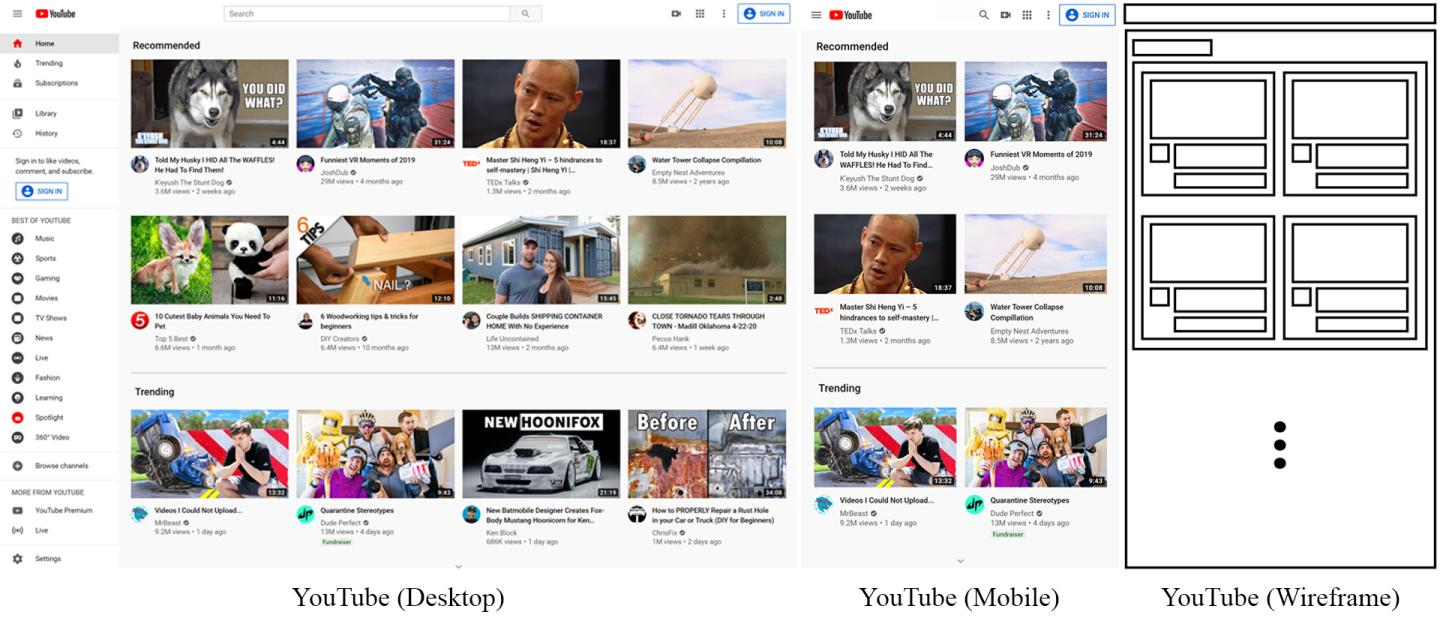
\includegraphics[width=1\textwidth]{src/youtube.jpg}
  \caption{Difference in Youtube Layout}
\end{figure}
When the viewer is using a desktop computer whose resolution width is higher than a threshold in pixels, the website shows the videos in 4 columns; when the viewer is using a mobile device with a much smaller width in pixels, however, the website shows the videos in 2 columns. To achieve this result, both the UI/UX designer and the application programmer have to do extra amount of work: the UI/UX designer must design multiple versions of the layout in different screen sizes, and the application programmer must write code that incorporates these layouts such that it renders correctly across all supported screen sizes. Specifically, the application programmer has to work out the parent-child relationships between the elements, known as the layout hierarchy. Unfortunately, this task is also time-consuming and error-prone, as the layout relationships are not immediately clear. For example, Figure 2 shows a simplified layout hierarchy of YouTube when rendered on a mobile device, in which the innermost element has a depth of 5. Along with even more complicated margins, this task poses a considerable challenge to the application programmer.
\paragraph{Our Work} In this paper, we present a proof-of-concept framework, named \W (Synthesizing responsive Webpage from Wireframe), to address the stated challenges. Specifically, we present the following technical contributions:
\W introduces a fast sectionalization algorithm to synthesize any absolute layout with hundreds of elements, specified by their absolute screen coordinates (x and y) and sizes (width and height), into a nested layout with hierarchical information inferred under a few milliseconds.
\W introduces a direct mapping of nested layouts to an HTML DOM (Document Object Model), exploiting the latest HTML5 features: flexboxes and grids. The resulting HTML can be rendered by any modern browser on its compatible devices.


\section{Related work}
There has been similar research in the area of generating layout code from images/rectangles. However; we did not find any work that comes too close to \textbf{W}$^2$: there is a machine-learning based approach to generate a web page from a mockup image [Huang et al. 2016], but it does not have a hierarchical layout specification; another approach aims to synthesize a relational layout\protect\footnote{ Note that "relational layout" is not the same as "hierarchical layout." In their work, the term "relational" refers to how the elements are relatively positioned against each other, i.e. the inter-element spacings.} for Android applications from a set of rectangles [Bielik et al. 2018], but it produces a flat hierarchy that relies on ConstraintLayout, a newly introduced feature in the newer versions of Android SDK, which is not as portable as HTML5 which is universal and cross-platform.

There is also work on generating UI layout for alternative screen orientation [Zeidler et al. 2017] and vectorizing UI screenshots [Swearngin et al. 2018]; but, once again, they did not target the web platform like \textbf{W}$^2$, which leverages HTML5 features to enable the resulting layout's responsiveness.

% Tiger

\section{Illustrative example}
When the wireframe is designed, we are given a static layout graph [Figure 2].
\begin{figure}[H]
  \vspace*{-0.1in}
  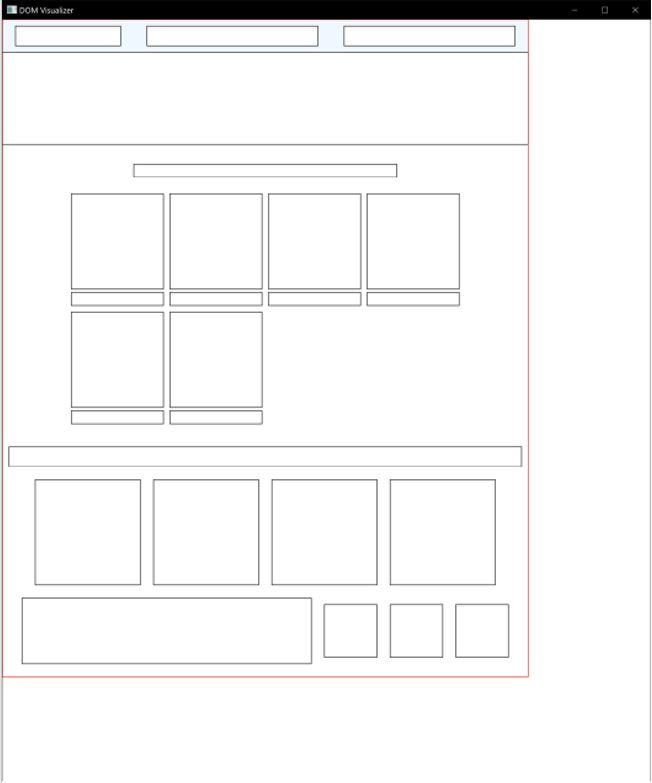
\includegraphics[width=0.5\textwidth]{src/wireframe.JPG}
  \caption{Static Wireframe Graph}
\end{figure}
We aim to transform this static layout to HTML script can directly run in browser. With the inference of the hierarchical structure by \textbf{W}$^2$, the website generated can adjust and adapt to various width [Figure 3]
\begin{figure}[H]
  \vspace*{-0.1in}
  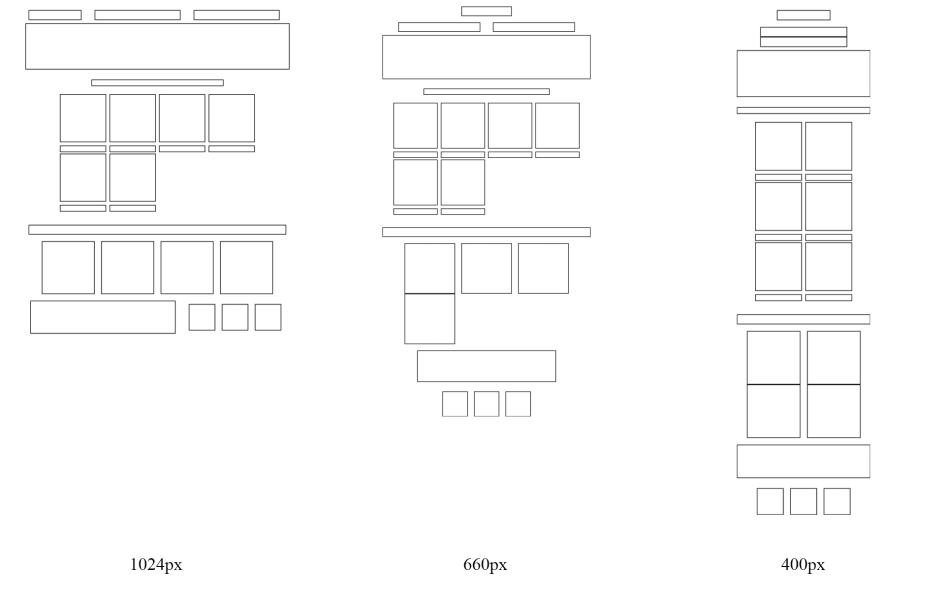
\includegraphics[width=1\textwidth]{src/compare.jpg}
  \caption{Responsive in Different Width}
\end{figure}

\section{Formal problem definition}
% Shangyin
In this work, we are given a list $L$, consisting of rectangles given their absolute coordinate with respective to origin. In addition, user provides the default size of the layout. All rectangles should be bounded by default size. Our objective is to find an equivalent HTML script which is: 
\begin{enumerate}
  \item \textbf{Precise -} Render the exact same layout when opened in  default size.
  \item \textbf{Responsive -} Automatically adjust the elements rendering if the browser is resized.
\end{enumerate}
\section{Preliminaries}
% Shangyin
\subsection{Workflow}
\begin{figure}[H]
  \vspace*{-0.1in}
  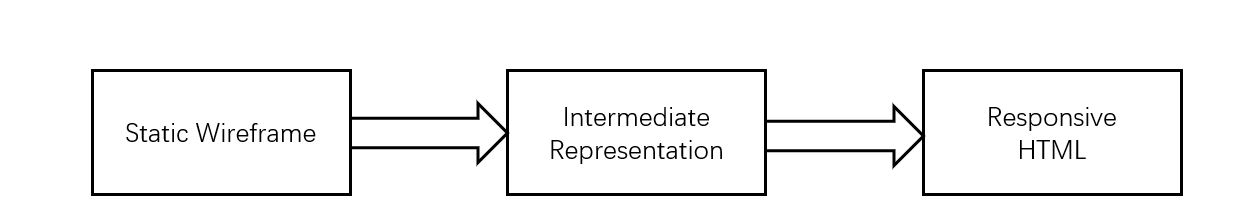
\includegraphics[width=1\textwidth]{src/workflow.JPG}
  \caption{Workflow}
\end{figure}
We define our workflow as a two-staged program. In the first stage, we synthesize the input Wireframe rectangles to IR. Then IR is compiled into universal HTML compatible with any browser in the second stage. 
\subsection{Input}
The input is defined as a list of rectangles, given their coordinates related to $(0,0)$, the upper-left corner of the canvas. For the consistency, we record the coordinates of the upper-left corner of a rectangle, as well as its width and height.
\subsection{IR Definition}
As discussed before, the intermediate presentation captures the nested hierarchy of raw rectangles. To maintain the hierarchical structure, we defined the data structure below.
\begin{figure}[H]
\vspace*{-0.2in}
\begin{lstlisting}[language=Scala,mathescape=true]
size = <Int, Int>
margin = <Int, Int, Int, Int>
Div = <size>
HDiv = <size, margin, VDiv*, Grid*, Div*>
VDiv = <size, margin, HDiv*, Grid*, Div*>
Grid = <size, margin, VDiv*, HDiv*, Div*>
Layout = Div | Grid | VDiv | HDiv
\end{lstlisting}
\caption{Definition of IR}
\end{figure}
We define \lstinline|Div| to be basic component of the hierarchy, which is equivalent to a raw rectangle in the input. All solid input rectangles are transformed into \lstinline|Div|s in different level of the tree in separate time during synthesizing. The three virtual containers for hierarchy are   \lstinline|HDiv|, \lstinline|VDiv|, \lstinline|GDiv|. As the name suggests, child containers of \lstinline|HDiv| and \lstinline|VDiv| are rendered in horizontal and vertical direction respectively. We define \lstinline|Grid| to behave like an HTML grid: two-dimensional container with auto row-wrapping. It contains homogenous elements, all rendered with same margin.


\section{Algorithm}
% Shangyin
In this section, we explain the procedures we used synthesizing the list of rectangles to IR with an estimate order of time complexity. We also present the compilation process from IR to final HTML result.
\subsection{IR Synthesis}
Recall that the input is a list of rectangles. This is the starting point of the synthesis, and we target the nested hierarchical IR. 

\subsubsection{Sectionalize} 
\begin{definition}{\lstinline{section}}
  We define a \lstinline{section} to be a set of rectangles which bounded by an inclusive lower bound $B_{low}$ and an inclusive upper bound $B_{up}$ in either $x$-direction or $y$-direction. In range $[B_{low}, B_{up}]$, we cannot find another bound $B_{mid}$ such that either $[B_{mid}, B_{up}]$ or $[B_{low}, B_{mid}]$ can form a \lstinline{section}.
\end{definition}

Given the list of rectangles, we divide such list into different \lstinline{section}s. To optimize the future operations, we want to find the max number of \lstinline{section}s. We propose the following sectionalize method.

\begin{figure}[H]
  \vspace*{-0.4in}
  \begin{lstlisting}[language=Scala,mathescape=true]

/*
Input - a list $L$ of rectangle
Output - a list $S$ of section
*/

sectionalize($L$: List[Rectangle]): List[section] = {
  val upperBounds = $L$.map(rectangles => rectangles.getUpperBound())
  val sectionBounds = upperBounds.filter(
    line => doesNotCutOtherRectangle(line))
  var $S$ = List()
  for (sectionLine <- sectionBounds) {
    $S$ = S + getRectangleBetween(sectionLine, lastSectionLine)
  }
  return $S$ 
}
  \end{lstlisting}
\caption{Sectionalize}
\end{figure}
In the above method, we first filter all upper-bounds of rectangles that does not go through other rectangles. Then, we argue that these lines are the bounds of that maximize the number of \lstinline{section}s. The proof is trivial and omitted. In each \lstinline{section}, we iterate through list $L$ and find all rectangles belong to this \lstinline{section}. Note that no specified direction is used in the above method, so it applies to both horizontal and vertical direction: we can sectionalize $L$ based on $x$ or $y$ coordinate.

Note that every \lstinline{section} can be easily converted into a \lstinline{VDiv} or \lstinline{HDiv}. We calculate the margin of each child rectangle of the \lstinline{section} by calculating the difference between that rectangle's coordinate and \lstinline{section} origin, which can be obtained by finding intersection of $B_{low}$ and outer coordinate.

Before the sectionalize operation, every rectangle is in the same level and container: every individual rectangle will be rendered with same priority and order. After we sectionalize a set of rectangles, we increase the depth of the hierarchy tree by $1$. Now each rectangle must belong to one \lstinline{section}. If we view each \lstinline{section} as an individual component, there will be another virtual \textit{master} container that contains all the \lstinline{section}s, which is visualized in the following graph,

\subsubsection{FormGrid} The central part of forming and optimizing the hierarchy relation is to identify \lstinline{Grid} from \lstinline{section}s. We see that in the previous sectionalize method, we generate a suboptimized hierarchical strucuture as we can put every rectangle into different \lstinline{VDiv} and \lstinline{HDiv} after sectionalizing. To further optimize the previous result, we want to merge different \lstinline{section}s into one \lstinline{Grid}.

For every \lstinline{section}, we classify the \lstinline{section} into \textit{simple} and \textit{complex} lists. We define \textit{simple} \lstinline{section} to be the section that contains only similar rectangles and are able to form \lstinline{Grid}. \textit{Complex} \lstinline{section} is cannot merge with other \lstinline{section} to form \lstinline{Grid} but can contain \lstinline{Grid}. 
% \begin{figure}[H]
%   \vspace*{-0.1in}
%   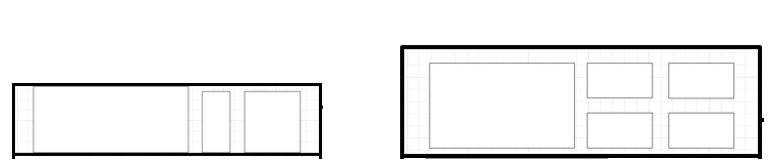
\includegraphics[width=1\textwidth]{src/simplevscomplex.JPG}
%   \caption{Workflow}
% \end{figure}


Then we iterate through the list of \lstinline{section}s and enumerates all possible of combination of \lstinline{section}s. We group larger \lstinline{Grid} first and then process smaller ones. For the \lstinline{section} fail to merge with other \lstinline{section}, we put them into the \textit{complex} \lstinline{section} for future processing.

\subsubsection{Complex Section}
\textit{Complex} \lstinline{section} indicates the need for further processing. The nature of web-page rendering suggests that elements are either arranged horizontally or vertically. Therefore, if the \textit{complex} \lstinline{section} was sectionalized based on $x$-coordinate, we now sectionalize it based on $y$-coordinate and vice versa. Within each \textit{complex} \lstinline{section}, we perform the above sectionalize and formGrid operation recursively until we meet max-depth or a single \lstinline{Div}.

In each execution of sectionalize and formGrid operation, we increase the depth of the hierarchy tree by 1. The result tree after termination is the IR we get and then feed into the IR-HTML compiler.
There are rare cases where the hierarchy tree produced fail to be optimal layout. We will discuss in future sections.

% \subsubsection{Input}
% RECT\\
% RECTLIST:= RECTLIST RECT | Nil
% \subsubsection{IR}
% DIV\\
% HDIV:= HDIV|DIV|VDIV\\
% VDIV:= HDIV|DIV|VDIV\\
% First we divide the rectangles into section based on their $y$-axis. Then we use
% greedy to find the earliest possible cut $y$ such that this $y$ does not divide any
% other rects.


\section{Evaluation}
We ran \W on a small set of representative test cases (|s|=5). Test case 1 to 3 are simple layouts; test case 4 is a design that is close to that in a real-world scenario (most rectangles are irregularly aligned, multiple layers of depth), and test case 5 is for stress testing (> 200 rectangles). The results are as below:
\begin{figure}[H]
  \vspace*{-0.1in}
  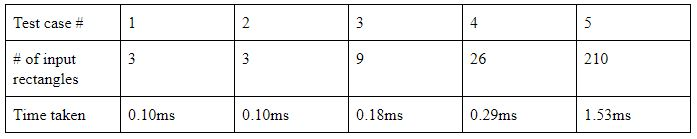
\includegraphics[width=1\textwidth]{src/benchmark.JPG}
  \caption{Benchmark}
\end{figure}
As our algorithm has a very limited search space and most UI layouts have fewer than 100 elements, it runs extremely fast—much faster than most similar work. Also, unlike neural-network based methods that often generate code that is non-interpretable or syntactically incorrect, \W produces a clean and robust DOM tree that is ready for display in the browser and easy to modify.

However, there are some limitations with \textbf{W}$^2$. For example, for a layout shown in Figure X, there exists two possible ways to sectionalize the layout, and \W always chooses the latter, due to its nature of returning the hierarchical tree of maximized depth. In the practical sense, though, the former sectionalization is more common as most websites adapt a multi-column layout. We have yet to clearly define a user-customizable parameter to measure the optimality of our synthesized hierarchy; hence, the resulting layout may not match the user's intent.
\begin{figure}[H]
  \vspace*{-0.1in}
  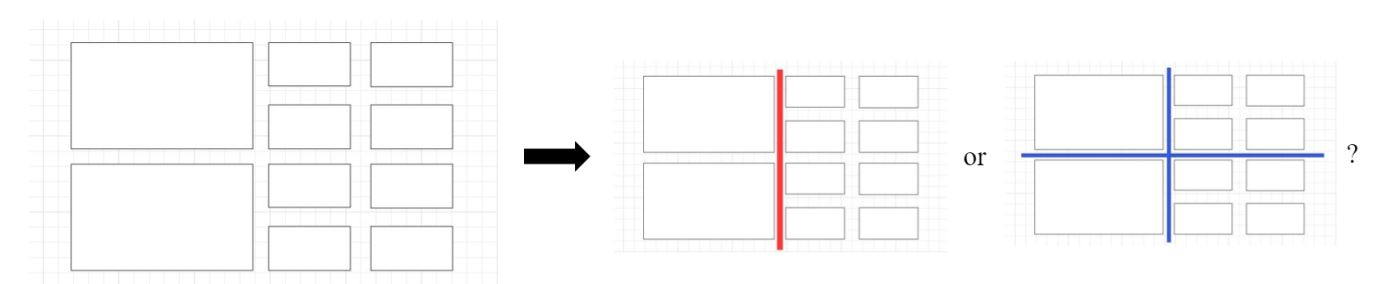
\includegraphics[width=1\textwidth]{src/limit.JPG}
  \caption{Benchmark}
\end{figure}


\section{Conclusion}
% Tiger

\end{document}